\documentclass{standalone}

\usepackage{tikz}

\usetikzlibrary{positioning, chains, shapes.geometric, fit, shapes, arrows.meta, calc}

\begin{document}

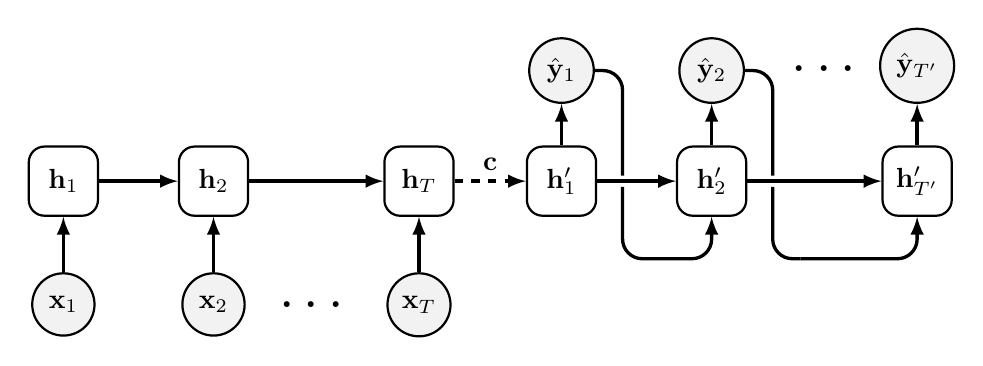
\begin{tikzpicture}[
    >=LaTeX, % Use default LaTeX arrows
    % Styles 
    cell/.style={ % RNN cell
        rectangle,
        rounded corners=2mm,
        minimum height=2.5em,
        minimum width=2.5em,
        draw,
        thick
    }, 
    cellc/.style={ % RNN cells in a chain
        cell,
        on chain,
        join
    },
    input/.style={ % Input or output node
        circle,
        minimum width=2.25em,
        draw,
        fill=gray!10,
        thick
    },
    arrow/.style={
        -latex,
        very thick
    },
    arrowc1/.style={ % Arrows with rounded corners
        arrow,
        rounded corners=.25cm
    },
    arrowc2/.style={ % Arrows with big rounded corners
        arrow,
        rounded corners=.5cm
    }
]

    % Encoder RNN
    \begin{scope}[start chain=going right, nodes=cellc, arrow, local bounding box=chain]
        \path[shift={(-9em, 1em)}] 
            node (h1) {$\mathbf{h}_1$}
            node[] (h2) {$\mathbf{h}_2$}
            node[xshift=2em] (hT) {$\mathbf{h}_{T}$};
    \end{scope}

    % Decoder RNN
    \begin{scope}[start chain=going right, nodes=cellc, arrow, local bounding box=chain]
        \path[shift={(9em, 1em)}] 
            node (h'1) {$\mathbf{h}'_1$}
            node[] (h'2) {$\mathbf{h}'_2$}
            node[xshift=2em] (h'T) {$\mathbf{h}'_{T'}$};
    \end{scope}

    % Context vector
    \draw[arrow, dashed] (hT) -- (h'1) node[midway, above] {$\mathbf{c}$};

    % Inputs and arrows from inputs
    \foreach \X in {1, 2} {
        \draw[arrow, latex-] (h\X.south) -- ++ (0, -2em)
            node[below, input] (x\X) {$\mathbf{x}_\X$};
    }
    \draw[arrow, latex-] (hT.south) -- ++ (0, -2em)
        node[below, input] (xT) {$\mathbf{x}_{T}$};

    % Outputs and arrows to outputs
    \draw[arrow] (h'1.north) -- ++ (0,1.5em)
        node[above, input] (y1) {$\hat{\mathbf{y}}_1$};
    \draw[arrow] (h'2.north) -- ++ (0,1.5em)
        node[above, input] (y2) {$\hat{\mathbf{y}}_2$};
    \draw[arrow] (h'T.north) -- ++ (0,1.5em)
        node[above, input] (yT) {$\hat{\mathbf{y}}_{T'}$};

    % Arrows from previous output to current output
    \draw[arrowc1, -] (y1.east) -| ++ (1em,-3.8em);
    \draw[arrowc1, -] (y1.east) ++ (1em,-4.2em) |- ++ (1em,-2.6em);
    \draw[arrowc1, -latex] (y1.east) ++ (2em,-6.8em) -| (h'2.south);

    \draw[arrowc1, -] (y2.east) -| ++ (1em,-3.8em);
    \draw[arrowc1, -] (y2.east) ++ (1em,-4.2em) |- ++ (1em,-2.6em);
    \draw[arrowc1, -latex] (y2.east) ++ (2em,-6.8em) -| (h'T.south);
    
    % Continuation dots
    \path (x2) -- (xT) node[midway, scale=2] {\dots};
    \path (y2) -- (yT) node[midway, scale=2, xshift=0.3em] {\dots};
\end{tikzpicture}

\end{document}